\subsection{Grandmother number-units}
\lipsum[1]

\begin{figure}[t]
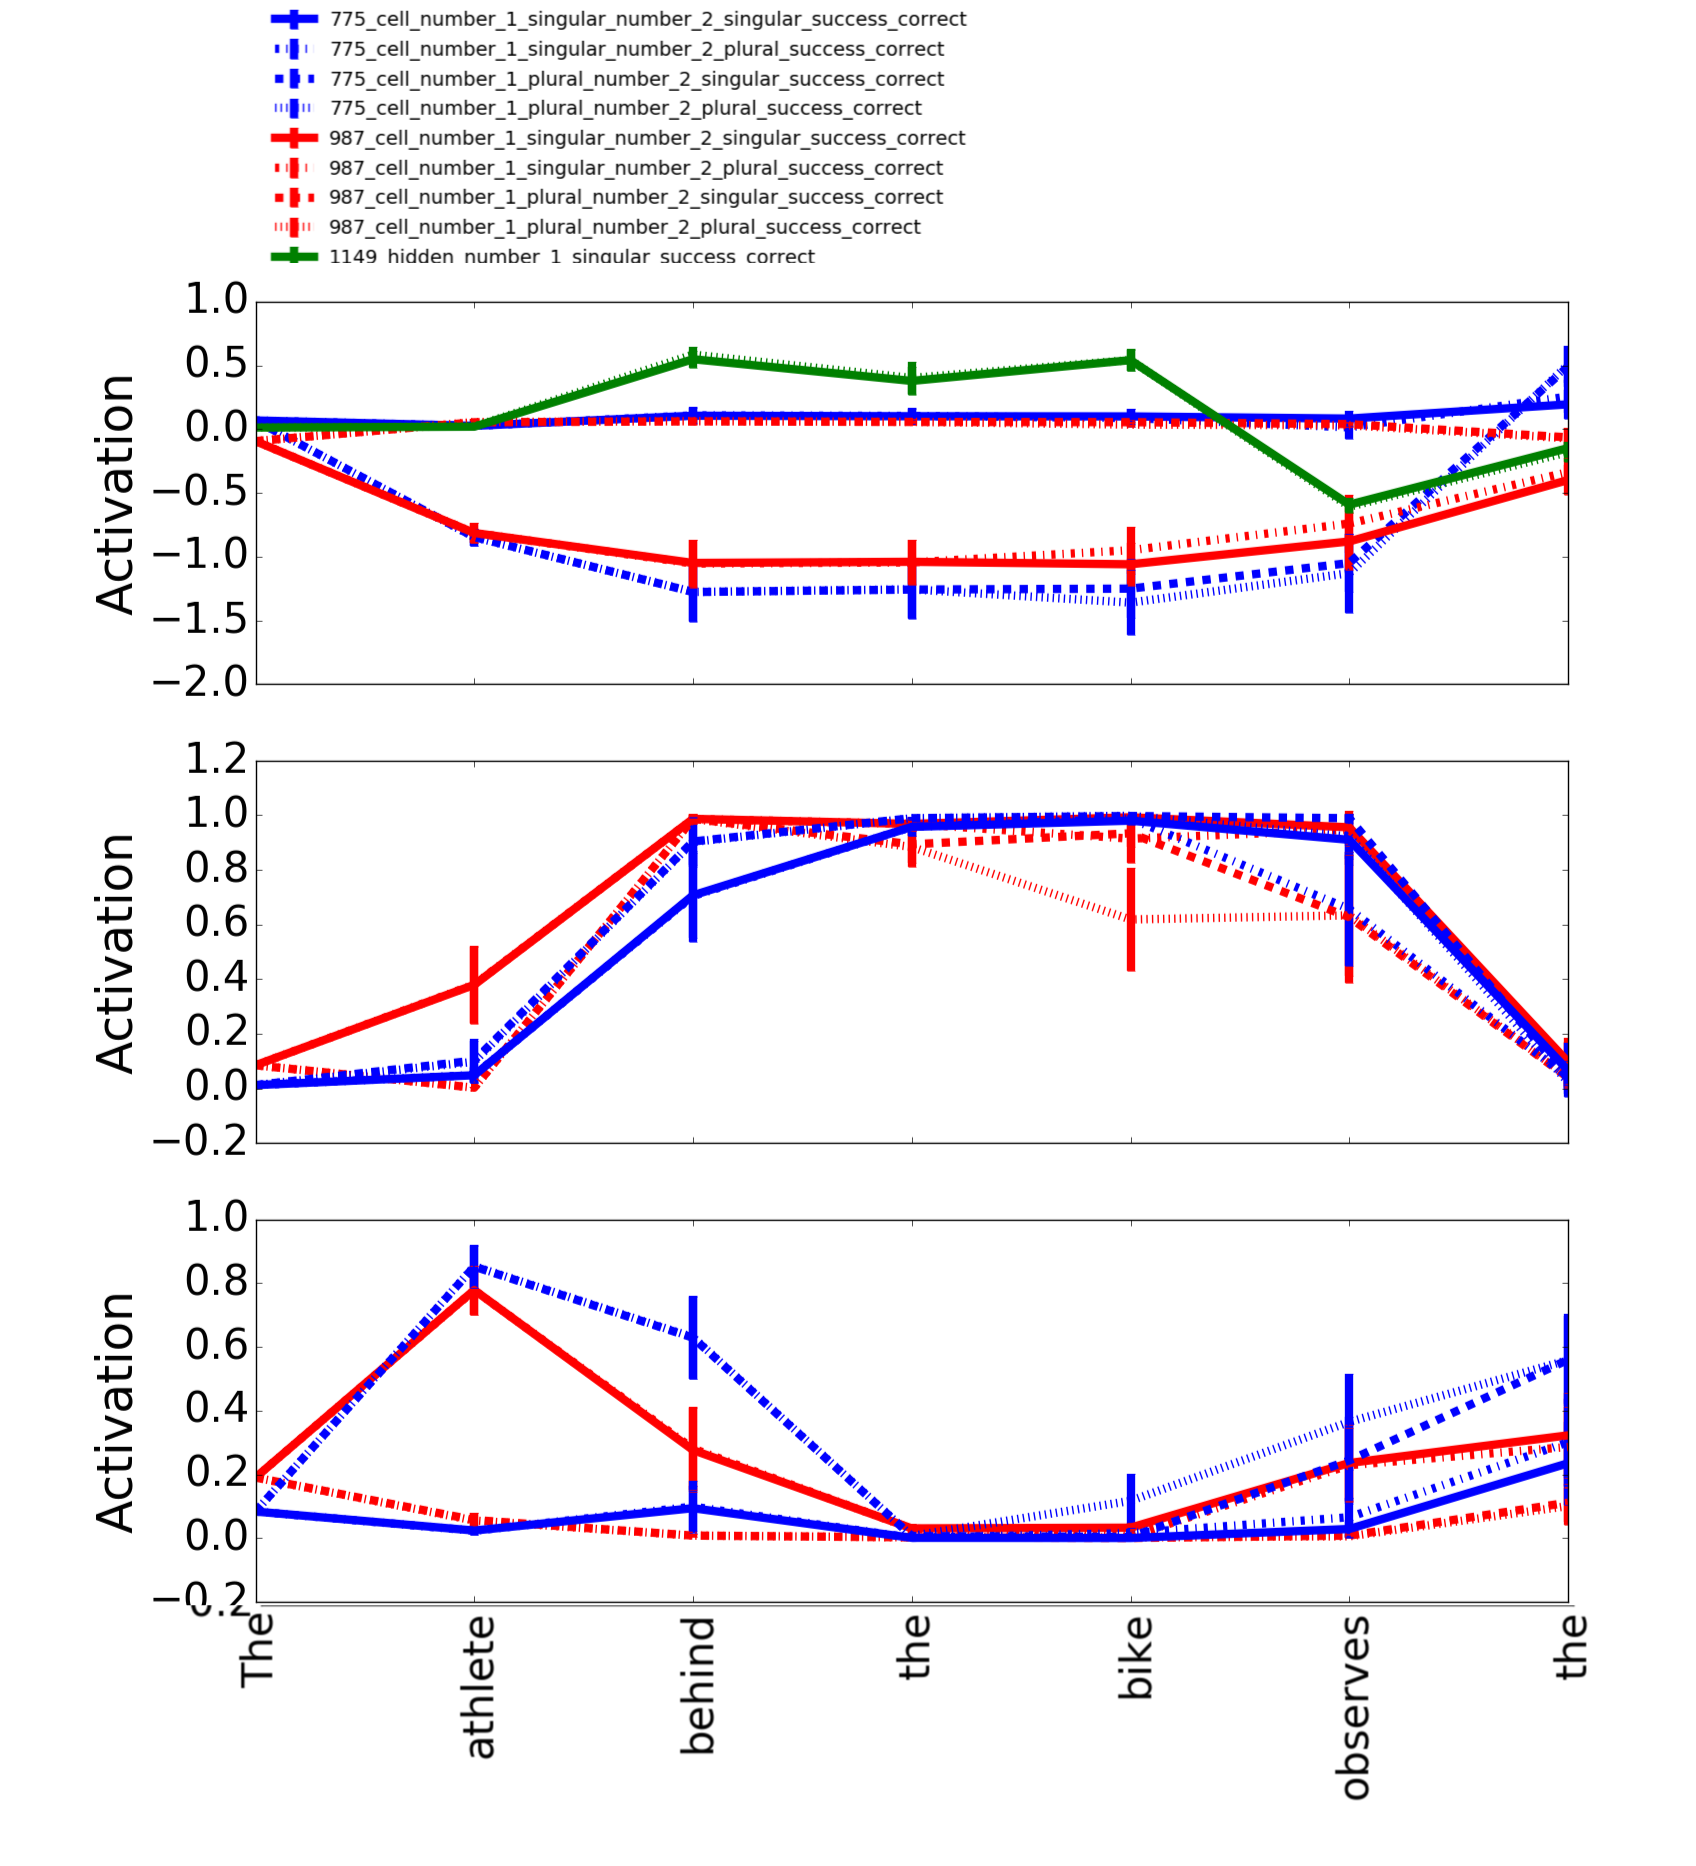
\includegraphics[width=\linewidth]{Figures/Figure2_number_units.png}
\caption{Cell and gate activations during processing of a sentence with a prepositional phrase between subject and verb. (A) Cell activity $C_t$ for the two number units 775 and 987 and output activity $h_t$ for the syntax unit 1149, for all four combinations of grammatical numbers of the two nouns. Note that the cell activity of units 775/987 is non-zero only when the first noun is plural/singular, respectively. (B) Corresponding forget-gate activity for the same number units. Note that gate activity is indifferent of the grammatical number of both nouns and that its value is close to one during the PP until after the verb. (C) Input-gate activity of the same units. Note that the gate value of unit 775/987 spikes around the first noun only when it is plural/singular.}
\end{figure}

\lipsum[1]

\begin{figure}
\centering
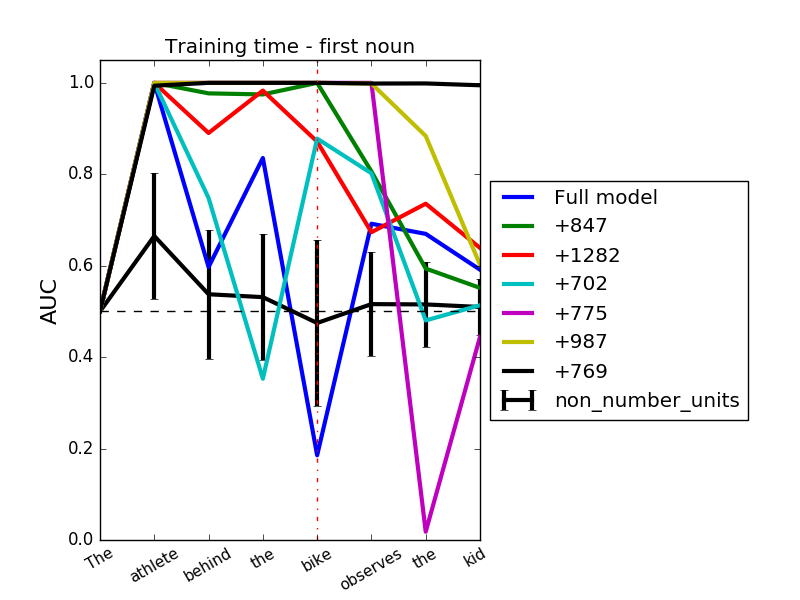
\includegraphics[width=\linewidth]{Figures/Figure3_number_units_GAT.png}
\caption{Generalization across time. To test whether the grammatical number of the first noun can be decoded from units activity at different time points, a linear-SVM was trained on unit activations $h_t$ at the time step of the first noun and then evaluated on all other time points. Area Under of Curve (AUC) values are shown for several cases: decoding from all LSTM units (full-model, black), a single number unit (775, purple; 1282, red...), average across all non-number units (black, error-bars represent standard-deviation). Note that the decoding of first-noun number is significantly higher from number units compared to all other units ($p-value<0.$).}
\end{figure}

\lipsum[1]

\begin{figure*}[t]
\centering
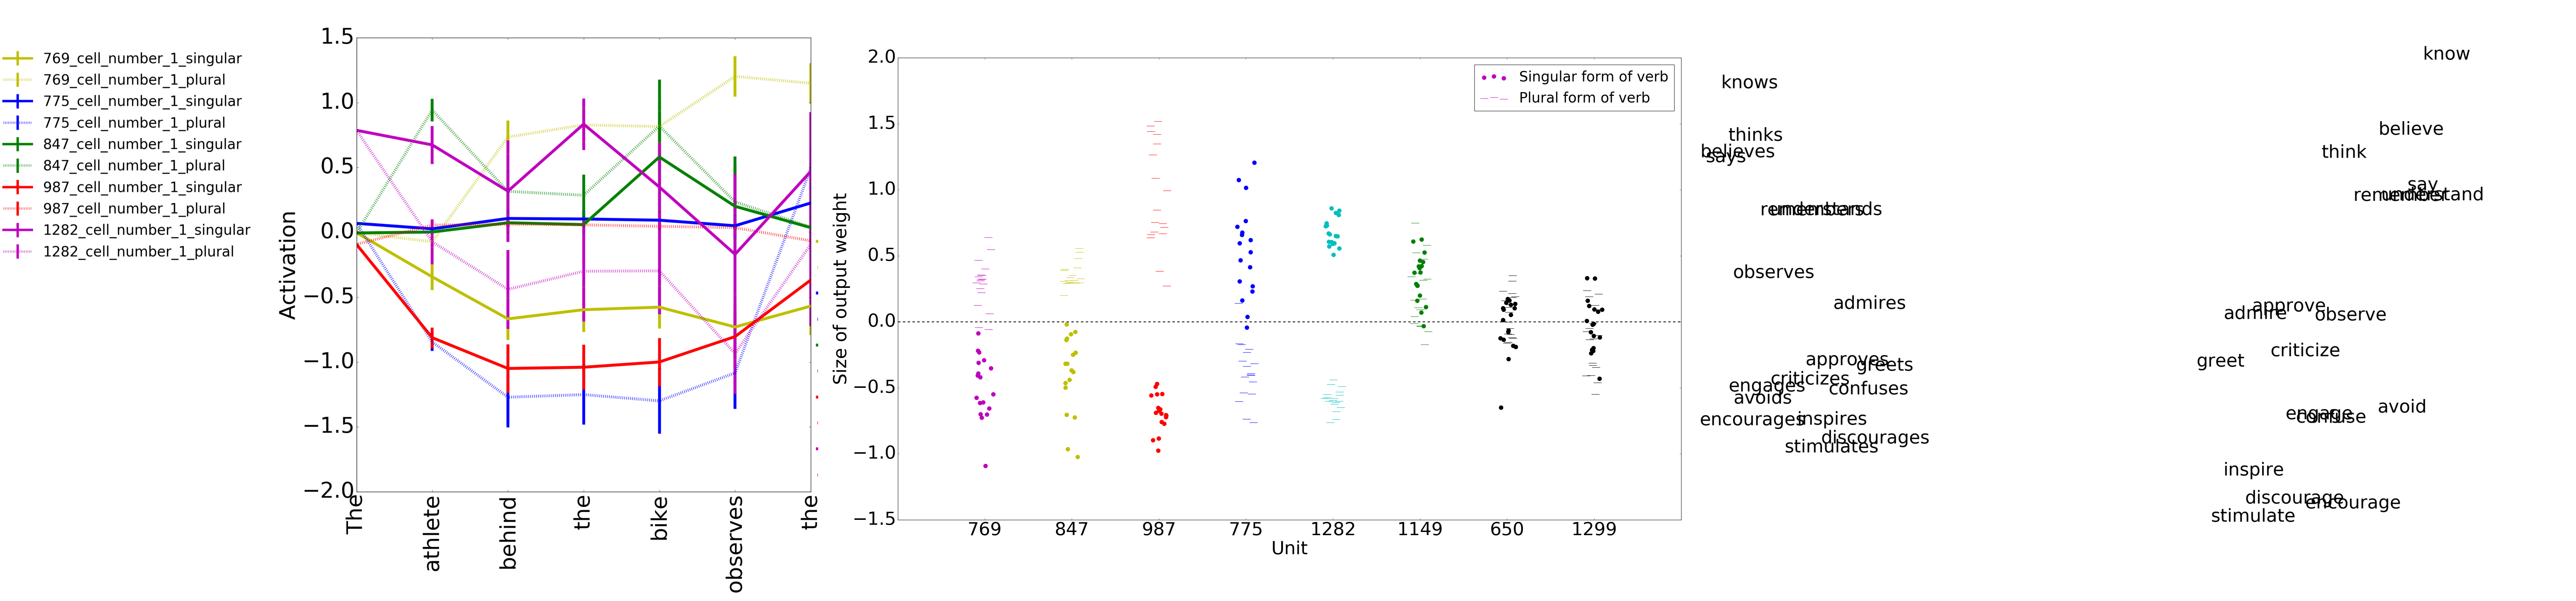
\includegraphics[width=\textwidth]{Figures/Figure4_output_weights.png}
\caption{Connectivity structure to output layer. (A) Output activity $h_t$ of all number units during the processing of a sentence with a PP between subject and verb. (B) Weight values from various units to output layer. Note that only for number units the output weights are clearly separated between singular and plural form of the verb, either positive or negative, compare to the syntax unit (1149) and two non-number units in the second layer. (C) Visualization of 18 verbs in their plural and singular forms (36 words in total) on the plane spanned by the two first principal components of their embeddings by the output weight matrix. A clear separation is observed between the singular and plural form along the first PC.}
\end{figure*}

\lipsum[1]

\subsubsection{Ablation study}
\lipsum[1]

\begin{figure}[b]
\centering
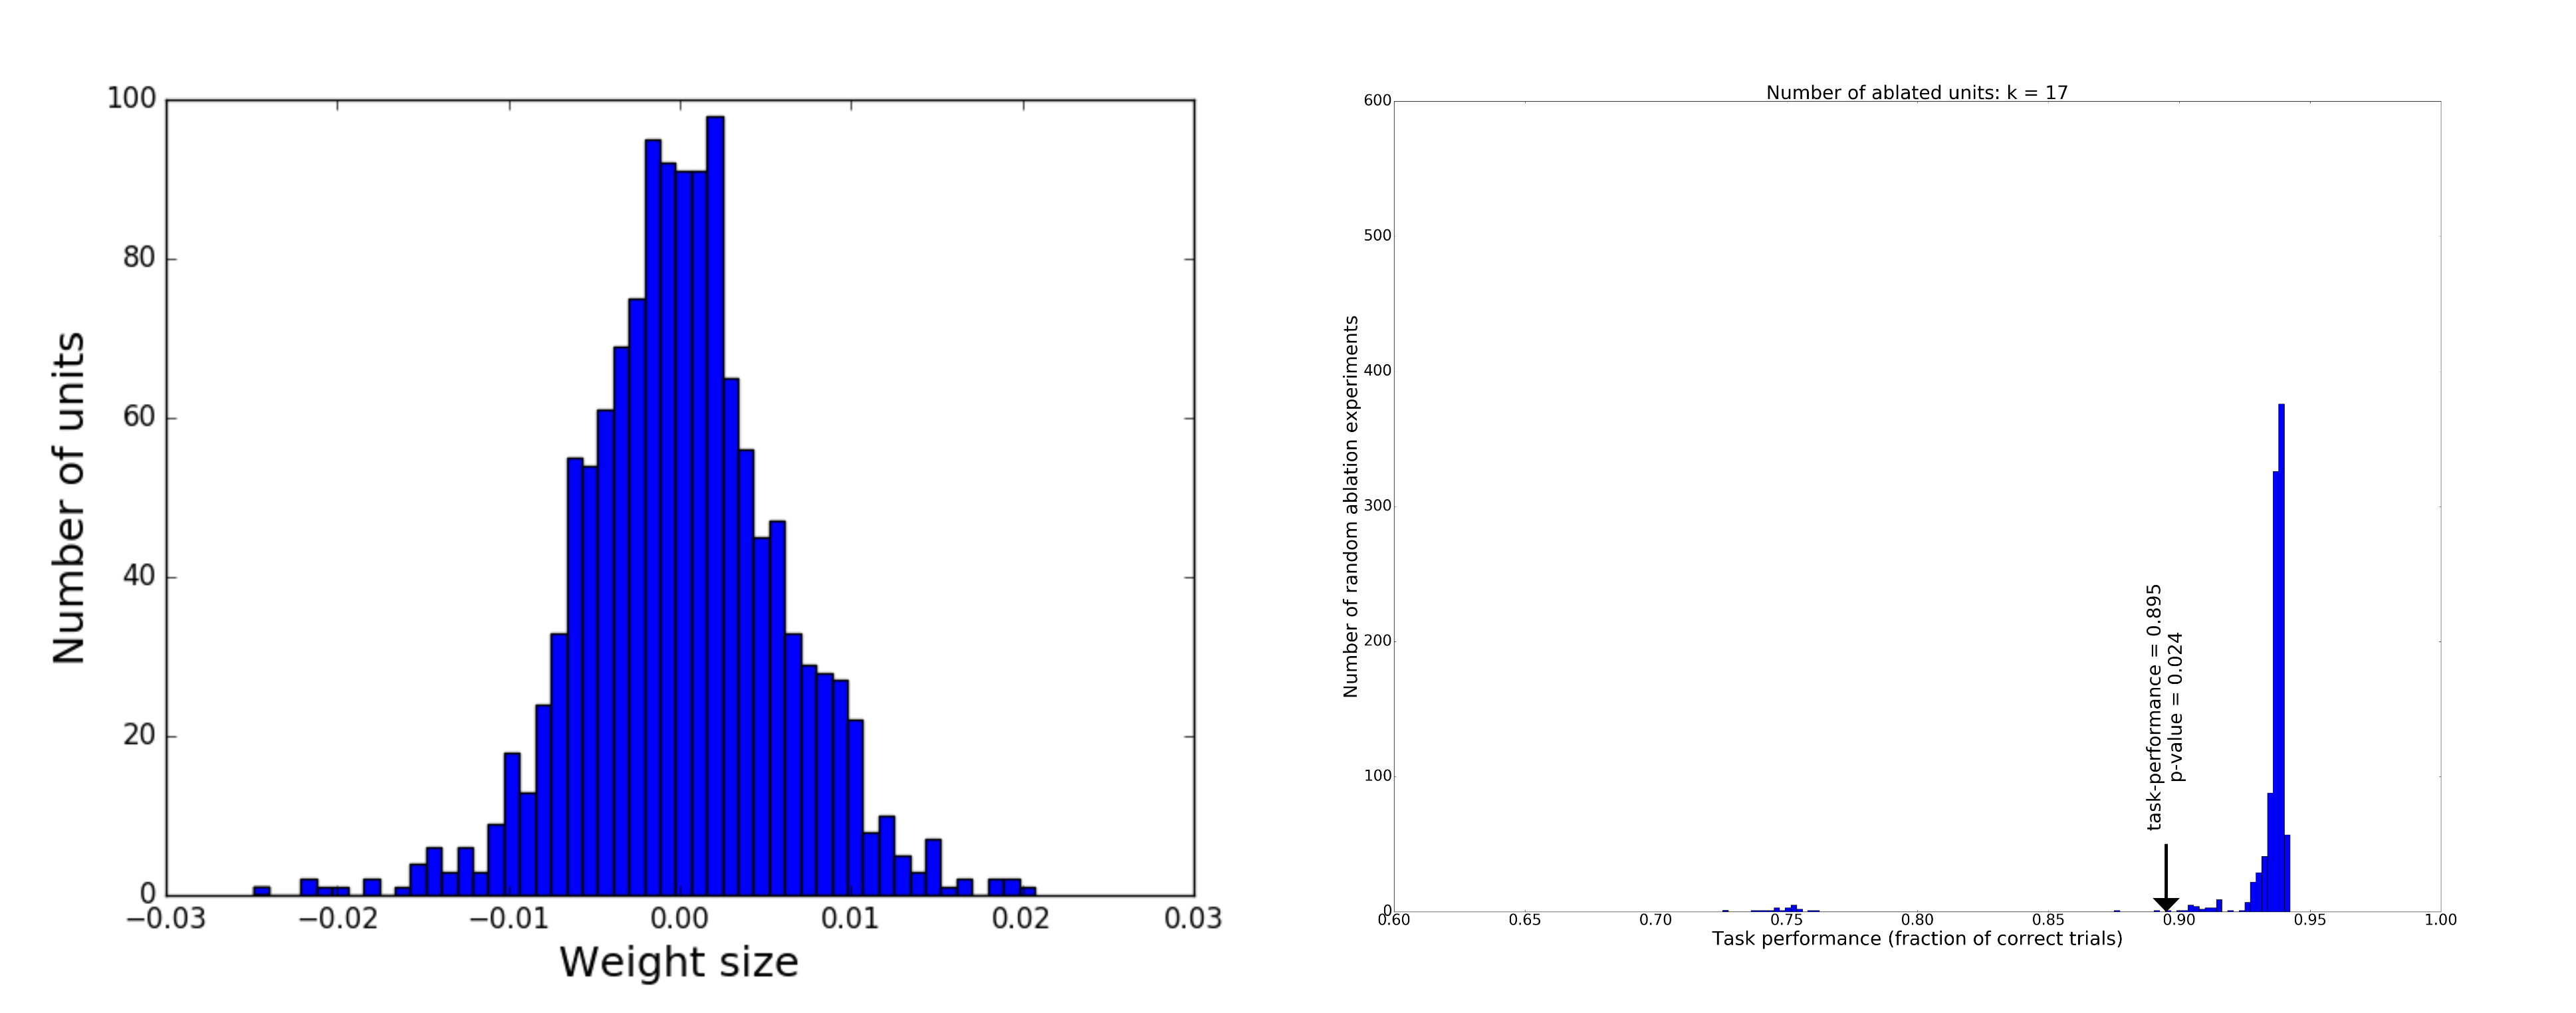
\includegraphics[width=\linewidth]{Figures/Figure6_regression.png}
\caption{(A) Distribution of the resulting weight values from the tree-depth regression model. Outlier weights were defined as having a value that is distant from the mean by more than three standard deviations (17 outlier weights in total - marked in red). (B) Task performance of 1000 models after ablating 17 random units (in blue) and based on the 17 outlier weights from the tree-depth regression model (black arrow). The reduction in performance due to outlier-weights ablation is statistically significant ($p-value < 0.05$) when compared to the null distribution generated by the random ablations.}
\end{figure}

\subsubsection{Visualizing unit dynamics}
\lipsum[1]

\subsubsection{Predicting the verb form}
Output weights + PCA
\lipsum[1]
